\hypertarget{index_overview}{}\section{Elektra Initiative Overview}\label{index_overview}
Elektra provides a universal and secure framework to store configuration parameters in a global, hierarchical key database. The core is a small library implemented in C. The plugin-\/based framework fulfills many configuration-\/related tasks to avoid any unnecessary code duplication across applications while it still allows the core to stay without any external dependency. Elektra abstracts from cross-\/platform-\/related issues with an consistent A\-P\-I, and allows applications to be aware of other applications' configurations, leveraging easy application integration.

See the website for more information \href{http://www.libelektra.org}{\tt http\-://www.\-libelektra.\-org}\hypertarget{index_focus}{}\section{A\-P\-I docu}\label{index_focus}
This document occupies with the A\-P\-I implementation, documentation, internals and plugins. On the one hand it gives an overview and an introduction for developers using Elektra, on the other hand it gives an informal descriptions what methods must and may provide to allow an alternative implementation of the A\-P\-I.

The current version (for stable releases) of this document can be found at \href{http://doc.libelektra.org/api/current/html}{\tt http\-://doc.\-libelektra.\-org/api/current/html}

The latest version (from git master) of this document can be found at \href{http://doc.libelektra.org/api/latest/html}{\tt http\-://doc.\-libelektra.\-org/api/latest/html}\hypertarget{index_using}{}\section{Using the Elektra Library}\label{index_using}
A C or C++ source file that wants to use Elektra should include\-: 
\begin{DoxyCode}
\textcolor{preprocessor}{#include <kdb.h>}
\end{DoxyCode}


To link an executable with the Elektra library, the correct way is to use the {\ttfamily pkg-\/config} tool\-: 
\begin{DoxyCode}
bash$ cc `pkg-config --libs elektra` -o myapp myapp.c
\end{DoxyCode}
\hypertarget{index_classes}{}\section{Elektra A\-P\-I}\label{index_classes}
The A\-P\-I was written in pure C because Elektra was designed to be useful even for the most basic system programs, which are all made in C. Also, being C, bindings to other languages can appear easily.

The A\-P\-I follows an Object Oriented design, and there are 3 main classes as shown by the figure\-:


\begin{DoxyImage}
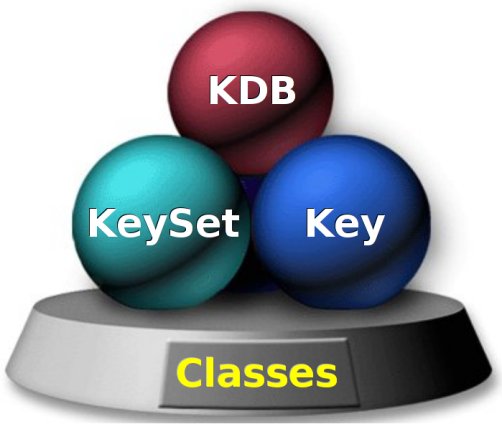
\includegraphics{classes.png}
\caption{Elektra Classes}
\end{DoxyImage}
 Some general things you can do with each class are\-:

\hyperlink{group__kdb}{K\-D\-B }
\begin{DoxyItemize}
\item \hyperlink{group__kdb}{The four lowlevel functions }
\item \hyperlink{group__kdb_ga6808defe5870f328dd17910aacbdc6ca}{Open } and \hyperlink{group__kdb_gadb54dc9fda17ee07deb9444df745c96f}{Close } the Database
\item \hyperlink{group__kdb_ga28e385fd9cb7ccfe0b2f1ed2f62453a1}{Get } and \hyperlink{group__kdb_ga11436b058408f83d303ca5e996832bcf}{Set } \hyperlink{group__keyset}{Key\-Set } in the Database
\item See \hyperlink{group__kdb}{class documentation} for more
\end{DoxyItemize}

\hyperlink{group__key}{Key }
\begin{DoxyItemize}
\item Get and Set key properties like \hyperlink{group__keyname_ga7699091610e7f3f43d2949514a4b35d9}{name }, \hyperlink{group__keyvalue_ga622bde1eb0e0c4994728331326340ef2}{string } or \hyperlink{group__keyvalue_gaa50a5358fd328d373a45f395fa1b99e7}{binary } values, \hyperlink{group__meta_gabc0cec592ce3b77e9bc33dbc8e8f6bdc}{permissions }, \hyperlink{group__meta_ga57689eb5691679071463b777ae786ae9}{changed time } and \hyperlink{group__meta_gafb89735689929ff717cc9f2d0d0b46a2}{comment }
\item Test if it is a \hyperlink{group__keytest_ga373acc20c6209357045891f4b0c70041}{{\ttfamily user/} } or \hyperlink{group__keytest_gafe49cfb61c2accb3073131c23a56fb14}{{\ttfamily system/} } key, etc
\item See \hyperlink{group__key}{class documentation} for more
\end{DoxyItemize}

\hyperlink{group__keyset}{Key\-Set }
\begin{DoxyItemize}
\item Linked list of Key objects
\item Append \hyperlink{group__keyset_gaa5a1d467a4d71041edce68ea7748ce45}{a single key } or an entire \hyperlink{group__keyset_ga21eb9c3a14a604ee3a8bdc779232e7b7}{Key\-Set }
\item \hyperlink{group__keyset_ga317321c9065b5a4b3e33fe1c399bcec9}{Work with } its \hyperlink{group__keyset_ga4287b9416912c5f2ab9c195cb74fb094}{internal cursor }
\item See \hyperlink{group__keyset}{class documentation} for more
\end{DoxyItemize}\hypertarget{index_keynames}{}\section{Key Names and Namespaces}\label{index_keynames}
There are 2 trees of keys\-: {\ttfamily system} and {\ttfamily user} 


\begin{DoxyItemize}
\item The \char`\"{}system\char`\"{} Subtree It is provided to store system-\/wide configuration keys, that is, configurations that daemons and system services will use. But all other programs will also try to fetch system keys to have a fallback managed by the distributor or admin when the user does not have configuration for its own.
\end{DoxyItemize}


\begin{DoxyItemize}
\item The \char`\"{}user\char`\"{} Subtree Used to store user-\/specific configurations, like the personal settings of a user to certain programs. The user subtree will always be favoured if present (except for security concerns the user subtree may not be considered). See \hyperlink{group__keyset_cascading}{Cascading} in the documentation of \hyperlink{group__keyset_gad2e30fb6d4739d917c5abb2ac2f9c1a1}{ks\-Lookup\-By\-Name()} how the selection of user and system keys works.
\end{DoxyItemize}\hypertarget{index_rules}{}\section{Rules for Key Names}\label{index_rules}
When using Elektra to store your application's configuration and state, please keep in mind the following rules\-:
\begin{DoxyItemize}
\item You are not allowed to create keys right under {\ttfamily system} or {\ttfamily user}. They are reserved for more generic purposes.
\item The keys for your application, called say {\itshape My\-App}, should be created under {\ttfamily system/sw/\-My\-App/current} and {\ttfamily user/sw/\-My\-App/current} 
\item current is the default configuration profile, users may symlink to the profile they want.
\item That means you just need to \hyperlink{group__kdb_ga28e385fd9cb7ccfe0b2f1ed2f62453a1}{kdb\-Get()} {\ttfamily system/sw/\-My\-App/profile} and {\ttfamily user/sw/\-My\-App/profile} and then \hyperlink{group__keyset_gad2e30fb6d4739d917c5abb2ac2f9c1a1}{ks\-Lookup\-By\-Name()} in {\ttfamily /sw/\-My\-App/profile} while profile defaults to current, but may be changed by the user or admin. See \hyperlink{group__keyset_cascading}{Cascading} to learn more about that feature.
\end{DoxyItemize}\hypertarget{index_backendsoverview}{}\section{Backend Overview}\label{index_backendsoverview}
The core of elektra does not store configuration itself to the harddisk. Instead this work is delegated to backends.

If you want to develop a backend, you should already have some experience with Elektra from the user point of view. You should be familiar with the data structures\-: \hyperlink{group__key}{Key } and \hyperlink{group__keyset}{Key\-Set } Then you can start reading about Backends, which are composed out of \hyperlink{group__plugin}{Plugins}.\hypertarget{index_glossary}{}\section{Glossary}\label{index_glossary}

\begin{DoxyItemize}
\item {\bfseries pop}, used in \hyperlink{group__keyset_gae42530b04defb772059de0600159cf69}{ks\-Pop()} and \hyperlink{group__keyset_KDB_O_POP}{K\-D\-B\-\_\-\-O\-\_\-\-P\-O\-P} means to remove a key from a keyset.
\item {\bfseries delete}, or abbr. del, used in \hyperlink{group__key_ga3df95bbc2494e3e6703ece5639be5bb1}{key\-Del()}, \hyperlink{group__keyset_ga27e5c16473b02a422238c8d970db7ac8}{ks\-Del()} and \hyperlink{group__keyset_gga98a3d6a4016c9dad9cbd1a99a9c2a45aa66a5380c120f25f28f49848c4a863ead}{K\-D\-B\-\_\-\-O\-\_\-\-D\-E\-L} means to free a key or keyset. The memory can be used for something else afterwards.
\item {\bfseries remove} means that the key/value information in the physical database will be removed permanently. 
\end{DoxyItemize}